\documentclass{beamer}\usepackage[]{graphicx}\usepackage[]{color}
%% maxwidth is the original width if it is less than linewidth
%% otherwise use linewidth (to make sure the graphics do not exceed the margin)
\makeatletter
\def\maxwidth{ %
  \ifdim\Gin@nat@width>\linewidth
    \linewidth
  \else
    \Gin@nat@width
  \fi
}
\makeatother

\definecolor{fgcolor}{rgb}{0.345, 0.345, 0.345}
\newcommand{\hlnum}[1]{\textcolor[rgb]{0.686,0.059,0.569}{#1}}%
\newcommand{\hlstr}[1]{\textcolor[rgb]{0.192,0.494,0.8}{#1}}%
\newcommand{\hlcom}[1]{\textcolor[rgb]{0.678,0.584,0.686}{\textit{#1}}}%
\newcommand{\hlopt}[1]{\textcolor[rgb]{0,0,0}{#1}}%
\newcommand{\hlstd}[1]{\textcolor[rgb]{0.345,0.345,0.345}{#1}}%
\newcommand{\hlkwa}[1]{\textcolor[rgb]{0.161,0.373,0.58}{\textbf{#1}}}%
\newcommand{\hlkwb}[1]{\textcolor[rgb]{0.69,0.353,0.396}{#1}}%
\newcommand{\hlkwc}[1]{\textcolor[rgb]{0.333,0.667,0.333}{#1}}%
\newcommand{\hlkwd}[1]{\textcolor[rgb]{0.737,0.353,0.396}{\textbf{#1}}}%
\let\hlipl\hlkwb

\usepackage{framed}
\makeatletter
\newenvironment{kframe}{%
 \def\at@end@of@kframe{}%
 \ifinner\ifhmode%
  \def\at@end@of@kframe{\end{minipage}}%
  \begin{minipage}{\columnwidth}%
 \fi\fi%
 \def\FrameCommand##1{\hskip\@totalleftmargin \hskip-\fboxsep
 \colorbox{shadecolor}{##1}\hskip-\fboxsep
     % There is no \\@totalrightmargin, so:
     \hskip-\linewidth \hskip-\@totalleftmargin \hskip\columnwidth}%
 \MakeFramed {\advance\hsize-\width
   \@totalleftmargin\z@ \linewidth\hsize
   \@setminipage}}%
 {\par\unskip\endMakeFramed%
 \at@end@of@kframe}
\makeatother

\definecolor{shadecolor}{rgb}{.97, .97, .97}
\definecolor{messagecolor}{rgb}{0, 0, 0}
\definecolor{warningcolor}{rgb}{1, 0, 1}
\definecolor{errorcolor}{rgb}{1, 0, 0}
\newenvironment{knitrout}{}{} % an empty environment to be redefined in TeX

\usepackage{alltt}  % option [handout] for printing
%\includeonlyframes{c}

%%%%%%%%%%%%%%%%%%%%%%%%%%%%%%%%%%%%%%%%%%%%%%%%%%%%%%%%%%%%%%%%%%%%%%%%%%%%%%%%
%%% BEAMER THEME SETTINGS %%%%%%%%%%%%%%%%%%%%%%%%%%%%%%%%%%%%%%%%%%%%%%%%%%%%%%
%%%%%%%%%%%%%%%%%%%%%%%%%%%%%%%%%%%%%%%%%%%%%%%%%%%%%%%%%%%%%%%%%%%%%%%%%%%%%%%%

\mode<presentation>
{
  \usetheme{Boadilla}      % or try Darmstadt, Madrid, Warsaw, ...
  \usecolortheme{BerlinFU} % or try albatross, beaver, crane, ...
  %\useoutertheme{smoothbars}
  \useoutertheme[subsection=false]{smoothbars}
  \usefonttheme{default}  % or try serif, structurebold, ...
  \setbeamertemplate{navigation symbols}{}
  \setbeamertemplate{caption}[default]
  \setbeamertemplate{itemize items}[circle]
  \setbeamertemplate{itemize subitem}[triangle]
  \setbeamertemplate{itemize subsubitem}[triangle]
  \setbeamertemplate{section in toc}[circle]
  \setbeamertemplate{subsection in toc}[default]
  \setbeamercolor{footline}{fg=black,bg=white}
  %\setbeamercolor{section in head/foot}{bg=white}
  %{\leavevmode\leftskip=1.5em${\color{BrickRed}\bullet}$\hskip0.5em\inserttocsubsection\par}
   \makeatletter
  %\def\verbatim@font{\ttfamily}  % comment out if using knitr
\makeatother
  \setbeamertemplate{bibliography item}{}
}

% This is for creating frames with no header and number
\newcommand{\framenoheader}{\setbeamertemplate{headline}[default]}
\newcommand{\framenonumber}{
      \setbeamertemplate{footline}
        {
      \leavevmode%
      \hbox{%
      \begin{beamercolorbox}[wd=.333333\paperwidth,ht=2.25ex,dp=1ex,center]{author in head/foot}%
        \usebeamerfont{author in head/foot}\insertshortauthor~~(\insertshortinstitute)
      \end{beamercolorbox}%
      \begin{beamercolorbox}[wd=.333333\paperwidth,ht=2.25ex,dp=1ex,center]{title in head/foot}%
        \usebeamerfont{title in head/foot}\insertshorttitle
      \end{beamercolorbox}%
      \begin{beamercolorbox}[wd=.333333\paperwidth,ht=2.25ex,dp=1ex,right]{date in head/foot}%
        \usebeamerfont{date in head/foot}\insertshortdate{}\hspace*{2em}
        {\color{white}\insertframenumber{} / \inserttotalframenumber\hspace*{2ex}} %#turning this line into a comment, erases the frame numbers
      \end{beamercolorbox}}%
      \vskip0pt%
    }
}

% Backup slides counter
\newcommand{\beginbackup}{
   \newcounter{framenumbervorappendix}
   \setcounter{framenumbervorappendix}{\value{framenumber}}
}
\newcommand{\backupend}{
   \addtocounter{framenumbervorappendix}{-\value{framenumber}}
   \addtocounter{framenumber}{\value{framenumbervorappendix}} 
}

%%%%%%%%%%%%%%%%%%%%%%%%%%%%%%%%%%%%%%%%%%%%%%%%%%%%%%%%%%%%%%%%%%%%%%%%%%%%%%%%
%%% PACKAGES %%%%%%%%%%%%%%%%%%%%%%%%%%%%%%%%%%%%%%%%%%%%%%%%%%%%%%%%%%%%%%%%%%%
%%%%%%%%%%%%%%%%%%%%%%%%%%%%%%%%%%%%%%%%%%%%%%%%%%%%%%%%%%%%%%%%%%%%%%%%%%%%%%%%

\usepackage{changepage}  % to adjust margins
\usepackage{tikz}
\usetikzlibrary{decorations.pathreplacing}
\usepackage{multirow}
\usepackage{array}
\usepackage{amssymb}
\usepackage{amsmath}
	\DeclareMathOperator{\logit}{logit}
	\DeclareMathOperator{\Bin}{Bin}
	\DeclareMathOperator{\Mult}{Mult}
	\DeclareMathOperator{\Poi}{Poi}
	\DeclareMathOperator{\half}{\frac{1}{2}}
\usepackage{dsfont}  % for indicator variables \mathsds{1}
  \DeclareMathOperator{\indicator}{\mathds{1}}
\usepackage[makeroom]{cancel}
  \renewcommand{\CancelColor}{\color{fu-red}}
\usepackage{wrapfig}
\usepackage[english]{babel}
\usepackage[utf8x]{inputenc}
%\setbeamersize{text margin left=25pt,text margin right=25pt}
\usepackage{pifont}
  \newcommand{\cmark}{\ding{51}}
  \newcommand{\xmark}{\ding{55}}
	\renewcommand{\H}{\text{\normalfont H}}
	\renewcommand{\d}{\text{ \normalfont d}}
	\newcommand{\E}{\text{\normalfont E}}
	\newcommand{\N}{\text{\normalfont N}}
	\renewcommand{\P}{\text{\normalfont P}}
	\newcommand{\Var}{\text{\normalfont Var}}
	\newcommand{\Cov}{\text{\normalfont Cov}}
\usepackage{listings}
\lstset{frame=single,commentstyle=\color{BrickRed},columns=fixed,basicstyle=\ttfamily,
stringstyle=\color{Red},keepspaces=true,showstringspaces=false,
numbers=none}
\lstdefinestyle{Rcode}{backgroundcolor=\color[gray]{0.95}}
\usepackage[resetlabels,labeled]{multibib}
\newcites{Tools}{Stuff}
\newcites{HMC}{HMC}

%%%%%%%%%%%%%%%%%%%%%%%%%%%%%%%%%%%%%%%%%%%%%%%%%%%%%%%%%%%%%%%%%%%%%%%%%%%%%%%%
%%% PRESENTATION SETTINGS %%%%%%%%%%%%%%%%%%%%%%%%%%%%%%%%%%%%%%%%%%%%%%%%%%%%%%
%%%%%%%%%%%%%%%%%%%%%%%%%%%%%%%%%%%%%%%%%%%%%%%%%%%%%%%%%%%%%%%%%%%%%%%%%%%%%%%%

\title[I-priors]{I-priors in Bayesian Variable Selection: From Reproducing Kernel Hilbert Spaces to Hamiltonian Monte Carlo}
\author[Haziq Jamil]{\large{Haziq Jamil}}
\institute[LSE]{Social Statistics (Year 3)\\ London School of Economics \& Political Science}
\date[3 Nov 2016]{3 November 2016\\
\hspace{1cm}\\
Social Statistics Meeting\\
\hspace{1cm}\\
follow along at: \href{https://haziqjamil.github.io/}{\color{fu-red} \textbf{https://haziqjamil.github.io/}}}

%%%%%%%%%%%%%%%%%%%%%%%%%%%%%%%%%%%%%%%%%%%%%%%%%%%%%%%%%%%%%%%%%%%%%%%%%%%%%%%%
%%% BEGIN DOCUMENT %%%%%%%%%%%%%%%%%%%%%%%%%%%%%%%%%%%%%%%%%%%%%%%%%%%%%%%%%%%%%
%%%%%%%%%%%%%%%%%%%%%%%%%%%%%%%%%%%%%%%%%%%%%%%%%%%%%%%%%%%%%%%%%%%%%%%%%%%%%%%%
\IfFileExists{upquote.sty}{\usepackage{upquote}}{}
\begin{document}

%%%%%%%%%%%%%%%%%%%%%%%%%%%%%%%%%%%%%%%%%%%%%%%%%%%%%%%%%%%%%%%%%%%%%%%%%%%%%%%%
%%% USEFUL COMMANDS %%%%%%%%%%%%%%%%%%%%%%%%%%%%%%%%%%%%%%%%%%%%%%%%%%%%%%%%%%%%
%%%%%%%%%%%%%%%%%%%%%%%%%%%%%%%%%%%%%%%%%%%%%%%%%%%%%%%%%%%%%%%%%%%%%%%%%%%%%%%%

% knitr options


%%%%%%%%%%%%%%%%%%%%%%%%%%%%%%%%%%%%%%%%%%%%%%%%%%%%%%%%%%%%%%%%%%%%%%%%%%%%%%%%
%%% FRONT SLIDE %%%%%%%%%%%%%%%%%%%%%%%%%%%%%%%%%%%%%%%%%%%%%%%%%%%%%%%%%%%%%%%%
%%%%%%%%%%%%%%%%%%%%%%%%%%%%%%%%%%%%%%%%%%%%%%%%%%%%%%%%%%%%%%%%%%%%%%%%%%%%%%%%

\begin{frame}[plain]
	\addtocounter{framenumber}{-1}
	\titlepage
\end{frame}

%%%%%%%%%%%%%%%%%%%%%%%%%%%%%%%%%%%%%%%%%%%%%%%%%%%%%%%%%%%%%%%%%%%%%%%%%%%%%%%%
%%% TOC %%%%%%%%%%%%%%%%%%%%%%%%%%%%%%%%%%%%%%%%%%%%%%%%%%%%%%%%%%%%%%%%%%%%%%%%
%%%%%%%%%%%%%%%%%%%%%%%%%%%%%%%%%%%%%%%%%%%%%%%%%%%%%%%%%%%%%%%%%%%%%%%%%%%%%%%%

{
\framenoheader\framenonumber
\begin{frame}[noframenumbering]{Outline}
\tableofcontents[sections=1-5]
\end{frame}
}

%%%%%%%%%%%%%%%%%%%%%%%%%%%%%%%%%%%%%%%%%%%%%%%%%%%%%%%%%%%%%%%%%%%%%%%%%%%%%%%%
\section{Bayesian Variable Selection} %%%%%%%%%%%%%%%%%%%%%%%%%%%%%%%%%%%%%%%%%%
%%%%%%%%%%%%%%%%%%%%%%%%%%%%%%%%%%%%%%%%%%%%%%%%%%%%%%%%%%%%%%%%%%%%%%%%%%%%%%%%

\subsection{The I-prior Bayesian Variable Selection model}

\begin{frame}{The I-prior Bayesian Variable Selection model}

	\begin{itemize}

		\item For centred responses $y_i$ and standardised covariates $x_{i1}, \dots, x_{ip}$,
		\begin{align}\label{eq:ipriorbvs}
			\begin{gathered}
				y_i = {\color{fu-red}\gamma_1}\beta_1 x_{i1} + \dots + {\color{fu-red}\gamma_p}\beta_p x_{ip} + \epsilon_i \\
				\epsilon_i \sim \text{N}(0, \psi^{-1})  \\
				i=1,\dots,n\\
				\\
				\text{\underline{Priors}} \\
				\boldsymbol\beta \sim \N(\mathbf 0, \psi\boldsymbol\Lambda \mathbf X ^\top \mathbf X \boldsymbol\Lambda), \text{ where } \boldsymbol\Lambda = \text{diag}[\lambda_1, \dots, \lambda_p]\\
				{\color{fu-red}\gamma_j} \sim \text{Bern}(p_j), \ j=1,\dots,p \\
				\psi, \lambda_1^{-2}, \dots,  \lambda_p^{-2} \sim \Gamma(c,d) \\
			\end{gathered}
		\end{align}

		\item Use MCMC methods to sample from posterior using software such as JAGS. Interested in two things:

		\begin{itemize}
			\item Posterior model probabilities $\P[\boldsymbol \gamma=\boldsymbol \gamma'|\mathbf y]$ for model $\boldsymbol\gamma'$.
			\item Posterior inclusion probabilities $\P[\gamma_j=1|\mathbf y]$ for variable $X_j$.
		\end{itemize}

	\end{itemize}

\end{frame}

\begin{frame}{Why Bayesian Variable Selection?}
	Some criticisms
	\begin{itemize}
		\item The end-game of model selection is often prediction. If so, better methods exist e.g. Lasso
		\item Why not just put a reasonable prior?
		\item Unreliable Gibbs sampler - likely to get stuck in multiple modes.
	\end{itemize}

	\pause

	But actually,
	\begin{itemize}
		\item Sometimes there is a need to know what is the most plausible, interpretable, and parsimonious model.
		\item Valid applications in social sciences, but perhaps not the $p > n$ cases.
		\item Gibbs sampler not too terrible.
		\item For as many critics to this ``combinatorial approach'', there are equally as many proponents.
		\item Prediction through Bayesian model averaging.
	\end{itemize}
\end{frame}

\begin{frame}{Simulation results are good...}
	\frametitle<2>{...in comparison to: SSVS (George \& McCulloch, 1993)}
	\frametitle<3>{...in comparison to: KM (Kuo \& Mallick, 1998)}
	\frametitle<4>{...in comparison to: GVS (Dellaportas et. al., 2011)}
	\frametitle<5>{...in comparison to: Lasso (Tibshirani, 1994)}
	\vspace{-1mm}
	\begin{onlyenv}<1>
		\includegraphics[height=3.1in]{figure/sim5}
	\end{onlyenv}
	\begin{onlyenv}<2>
		\includegraphics[height=3.1in]{figure/sim1}
	\end{onlyenv}
	\begin{onlyenv}<3>
		\includegraphics[height=3.1in]{figure/sim2}
	\end{onlyenv}
	\begin{onlyenv}<4>
		\includegraphics[height=3.1in]{figure/sim3}
	\end{onlyenv}
	\begin{onlyenv}<5>
		\includegraphics[height=3.1in]{figure/sim6}
	\end{onlyenv}	
\end{frame}

\begin{frame}{...and so are some real world applications}
%	\vspace{-3mm}
%	I-priors perform equally well, and in some cases, better than various model selection techniques.

	\begin{itemize}\setlength\itemsep{0.8em}
		\item[1] \textbf{Modelling aerobic fitness through some exercise data} ($n = 30$, $p = 6$) [SAS/STAT User Guide, 2008]
			\begin{itemize}
				\item Agreed with forward selection and backward elimination procedure except in the \texttt{Age} variable.
				\item \texttt{Age} negatively correlated with \texttt{MaxPulse}.
			\end{itemize}
		\item[2] \textbf{Effects of air pollution on mortality rate} ($n = 60$, $p = 15$) [McDonald \& Schwing, 1978]
			\begin{itemize}
				\item Which of \texttt{HC}, \texttt{NOx}, and/or \texttt{SO2} affects mortality rate in U.S. metropolitan areas?
				\item Agreed with ``ridge trace analysis'' in identifying \texttt{SO2}.
			\end{itemize}
		\item[3] \textbf{Factors affecting ozone depletion} ($n = 178$, $p = 12,90$) [Casella \& Moreno, 2006]
			\begin{itemize}
				\item Model obtained had smaller out-of-sample RMSE.
				\item Selection of squared and two-way interaction terms to improve RMSE without overcomplicating the model.
			\end{itemize}
	\end{itemize}
\end{frame}

%%%%%%%%%%%%%%%%%%%%%%%%%%%%%%%%%%%%%%%%%%%%%%%%%%%%%%%%%%%%%%%%%%%%%%%%%%%%%%%%
\section{I-priors} %%%%%%%%%%%%%%%%%%%%%%%%%%%%%%%%%%%%%%%%%%%%%%%%%%%%%%%%%%%%%
%%%%%%%%%%%%%%%%%%%%%%%%%%%%%%%%%%%%%%%%%%%%%%%%%%%%%%%%%%%%%%%%%%%%%%%%%%%%%%%%

{
\framenonumber
\begin{frame}[noframenumbering]
	\tableofcontents[currentsection, sections=1-5, hideallsubsections]
\end{frame}
}

%%%%%%%%%%%%%%%%%%%%%%%%%%%%%%%%%%%%%%%%%%%%%%%%%%%%%%%%%%%%%%%%%%%%%%%%%%%%%%%%

\subsection{Introduction}

\begin{frame}{Introduction}
	\vspace{-4mm}

	\begin{itemize}
		\item For $i = 1, \dots, n$, consider the regression model
		\begin{align*}
			\begin{gathered}
				y_i = \alpha + f(\mathbf x_i) + \epsilon_i \\
				(\epsilon_1, \dots, \epsilon_n) \sim \N(\mathbf 0, \boldsymbol{\Psi}^{-1})
			\end{gathered}
		\end{align*}
		where $f \in \mathcal F$, $y_i \in \mathbb R$, and $\mathbf x_i = (x_{i1}, \dots, x_{ip}) \in \mathcal X$.

	\pause
	\item Definition \textbf{(I-priors)} \\
	\textit{For the regression model above, let $\mathcal F$ be a reproducing kernel Hilbert space (RKHS) with kernel $h_{\boldsymbol\lambda}: \mathcal X \times \mathcal X \rightarrow \mathbb R$. Then, assuming it exists, the Fisher information for $I[f]$ for the function $f$ is given by
		\[
		I[f(\mathbf x_i), f(\mathbf x_i')] = \sum_{k=1}^n \sum_{l=1}^n \psi_{kl} h_{\boldsymbol\lambda}(\mathbf x_i, \mathbf x_k) h_{\boldsymbol\lambda}(\mathbf x_i', \mathbf x_l).
		\]
		Let $\pi$ be a Gaussian distribution on the random vector $f$ with mean $f_0$ and covariance kernel $I[f]$. Then $\pi$ is called an I-prior for $f$.
	}
	\end{itemize}
\end{frame}

\begin{frame}{Function spaces and kernels}
	\begin{itemize}
		\item There is a bijection between the set of all positive-definite functions (reproducing kernels) $h:\mathcal X \times \mathcal X \rightarrow \mathbb R$ and the set of all RKHS.
	\end{itemize}

	\small{
	\renewcommand{\arraystretch}{1.3}
	\begin{table}[htdp]
	\begin{center}
	\begin{tabular}{m{1.15cm}|m{2.5cm}|m{2.7cm}|m{3.3cm}}
	$\tiny{\mathcal X \!=\! \{x_i\}}$	&\textbf{Effect}		&\textbf{Vector space} $\mathcal{F}$		&\textbf{Kernel} $h( x_i,  x_k)$ \\
	\hline
	Real		&\footnotesize{``Straight line'' \newline functions}
	&Canonical	&$x_ix_k$ \\
	\hline
	Real		&\footnotesize{``Curvy'' functions \newline (smoothing)}
	&Fractional Brownian Motion (FBM)	&\footnotesize{$|x_i|^{2\gamma} + |x_k|^{2\gamma} - |x_i - x_k|^{2\gamma}$ with $\gamma \in (0,1)$} \\
	\hline
	Nominal		&\footnotesize{Grouping}
	&Pearson	&$\frac{\indicator[x_i=x_k]}{p_i} - 1$ \newline \footnotesize{where $p_i = \text{P}[X = x_i]$} \\
	\end{tabular}
	\end{center}
	\label{default}
	\end{table}
	}

\end{frame}

\begin{frame}{The $w$ I-prior model}
	\vspace{-3mm}

	\begin{itemize}
		\item The I-prior for $f$ has the random-effect representation
		\begin{align*}
			\begin{gathered}
				f(\mathbf x_i) = \alpha + f_0(\mathbf x_i) + \sum_{k=1}^n h_{\boldsymbol\lambda}(\mathbf x_i, \mathbf x_k)w_k \\
				(w_1,\dots,w_n) \sim \N(\mathbf 0, \boldsymbol\Psi).
			\end{gathered}
		\end{align*}

		\item Putting this back into our regression model, we obtain the \textit{w I-prior} model
		\only<1>{
		\begin{align*}
			\begin{gathered}
				y_i = \alpha + f_0(\mathbf x_i) + \sum_{k=1}^n h_{\boldsymbol\lambda}(\mathbf x_i, \mathbf x_k)w_k + \epsilon_i \\
				(w_1, \dots, w_n) \sim \N(\mathbf 0, \boldsymbol{\Psi}) \\
				(\epsilon_1, \dots, \epsilon_n) \sim \N(\mathbf 0, \boldsymbol{\Psi}^{-1}) \\
			\end{gathered}
		\end{align*}
		}
		\uncover<2->{
		\begin{align*}
			\begin{gathered}
				\mathbf y = \boldsymbol\alpha + \mathbf f_0 + \mathbf H_{\boldsymbol\lambda} \mathbf w + \boldsymbol\epsilon \\
				\mathbf w \sim \N(\mathbf 0, \boldsymbol{\Psi}) \\
				\boldsymbol\epsilon \sim \N(\mathbf 0, \boldsymbol{\Psi}^{-1})
			\end{gathered}
		\end{align*}
		}

		\only<3>{
		\item Typically, $(\mathbf H_{\boldsymbol{\lambda}})_{ij} = \sum_{k=1}^p \lambda_k h_k(x_{ik}, x_{jk})$
		}

		\only<4>{
		\item Typically, $\mathbf H_{\boldsymbol{\lambda}} = \lambda_1 \mathbf H_1 + \cdots + \lambda_p \mathbf H_p$
		}

		\uncover<5->{
		\item Typically, $\mathbf H_{\boldsymbol{\lambda}} = \lambda_1 \mathbf H_1 + \cdots + \lambda_p \mathbf H_p$, $\boldsymbol{\Psi} = \psi\mathbf I_n$, and $\mathbf f_0 = \mathbf 0$.
		}

		\uncover<6->{
		\item Parameters of interest are $\boldsymbol{\theta} = (\alpha, \lambda_1, \dots, \lambda_p, \psi).$
		}
	\end{itemize}
\end{frame}

\subsection{Estimation}

\begin{frame}{Maximum likelihood}
	\begin{itemize}
		\item The marginal distribution of $\mathbf y$ is normal with mean and variance
		\begin{align*}
			\begin{gathered}
				\E[\mathbf y] = \boldsymbol\alpha \\
				\Var[\mathbf y] = \psi \mathbf  H_{\boldsymbol\lambda}^2 + \psi^{-1}\mathbf I_n =: \mathbf V_y
			\end{gathered}
		\end{align*}
		and thus, the marginal log-likelihood is given by
		\[
			l(\boldsymbol{\theta}) = - \frac{n}{2} \log(2\pi) - \frac{1}{2} \log | \mathbf V_y | - \frac{1}{2}  (\mathbf y - \boldsymbol\alpha)^\top \mathbf V_y^{-1} (\mathbf y - \boldsymbol\alpha).
		\]

		\item MLE for intercept is $\hat\alpha = \bar y = \frac{1}{n}\sum_{i=1}^n y_i$.
		\item Usually no closed form estimates for $\boldsymbol{\lambda}$ and $\psi$, so use numerical optimisation to find MLE.
		\item Problem: Convergence is difficult when there are a lot of scale parameters.
	\end{itemize}
\end{frame}

\begin{frame}{EM algorithm}
	\begin{itemize}
		\item A more stable method is using the EM algorithm. Treat the random effects $\mathbf w$ as ``missing''.
		\item The relevant distributions are easy enough to obtain:
		\begin{itemize}
			\item $\mathbf y \sim \N(\boldsymbol\alpha, \mathbf V_y)$ \vspace{1pt}
			\item $\mathbf w \sim \N(\mathbf 0, \psi\mathbf I_n)$ \vspace{3pt}
			\item $\begin{pmatrix}\mathbf y \\ \mathbf w\end{pmatrix} \sim \N\Bigg(\begin{pmatrix}\boldsymbol\alpha\\\mathbf 0\end{pmatrix}, \begin{pmatrix} \mathbf V_y & \mathbf \psi \mathbf H_{\boldsymbol\lambda} \\ \psi\mathbf H_{\boldsymbol\lambda} & \psi\mathbf I_n \end{pmatrix}\Bigg)$ \vspace{2pt}
			\item $\mathbf w | \mathbf y \sim \N\left(\psi\mathbf H_{\boldsymbol\lambda} \mathbf V_y^{-1} (\mathbf y - \boldsymbol\alpha), \mathbf V_y^{-1}\right)$
		\end{itemize}

		\item For $t = 0, 1, \dots$, do:
		\begin{itemize}
			\item E-step: Calculate $Q(\boldsymbol\lambda, \psi) = \text{E}_{\mathbf w} \left[\log f(\mathbf y, \mathbf w ; \boldsymbol\theta)  | \mathbf y; \boldsymbol\lambda^{(t)}, \psi^{(t)}, \hat\alpha \right]$.

			\item M-step: $(\boldsymbol\lambda^{(t+1)}, \psi^{(t+1)}) \gets \arg\max_{(\boldsymbol\lambda, \psi)} Q(\boldsymbol\lambda, \psi)$.
		\end{itemize}


		\item Problem: May be very slow to converge.
	\end{itemize}
\end{frame}

\subsection{The R/iprior package}

%%%%%%%%%%%%%%%%%%%%%%%%%%%%%%%%%%%%%%%%%%%%%%%%%%%%%%%%%%%%%%%%%%%%%%%%%%%%%%%%
%%% knitr iprior models %%%%%%%%%%%%%%%%%%%%%%%%%%%%%%%%%%%%%%%%%%%%%%%%%%%%%%%%
%%%%%%%%%%%%%%%%%%%%%%%%%%%%%%%%%%%%%%%%%%%%%%%%%%%%%%%%%%%%%%%%%%%%%%%%%%%%%%%%

\newsavebox{\ipriordemoa}
\begin{lrbox}{\ipriordemoa}
\begin{knitrout}\small
\definecolor{shadecolor}{rgb}{0.969, 0.969, 0.969}\color{fgcolor}\begin{kframe}
\begin{alltt}
\hlkwd{str}\hlstd{(hsbsmall,} \hlkwc{width} \hlstd{=} \hlnum{58}\hlstd{,} \hlkwc{strict.width} \hlstd{=} \hlstr{"cut"}\hlstd{)}
\end{alltt}
\begin{verbatim}
## 'data.frame':	661 obs. of  3 variables:
##  $ mathach : num  16.663 -2.155 0.085 18.804 2.409 ...
##  $ ses     : num  0.322 0.212 0.682 -0.148 -0.468 0.842 ..
##  $ schoolid: Factor w/ 16 levels "1374","1433",..: 1 1 1..
\end{verbatim}
\end{kframe}
\end{knitrout}
\end{lrbox}

\newsavebox{\ipriordemoaa}
\begin{lrbox}{\ipriordemoaa}
\begin{knitrout}\small
\definecolor{shadecolor}{rgb}{0.969, 0.969, 0.969}\color{fgcolor}\begin{kframe}
\begin{alltt}
\hlkwd{str}\hlstd{(hsbsmall)}
\end{alltt}
\end{kframe}
\end{knitrout}
\end{lrbox}

\newsavebox{\ipriordemob}
\begin{lrbox}{\ipriordemob}
\begin{knitrout}\small
\definecolor{shadecolor}{rgb}{0.969, 0.969, 0.969}\color{fgcolor}\begin{kframe}
\begin{alltt}
\hlkwd{system.time}\hlstd{(}
  \hlstd{mod} \hlkwb{<-} \hlkwd{iprior}\hlstd{(mathach} \hlopt{~} \hlstd{ses,} \hlkwc{data} \hlstd{= hsbsmall)}
\hlstd{)}
\end{alltt}
\begin{verbatim}
## Iteration 0:    Log-likelihood = -19755.905 .......
## Iteration 100:  Log-likelihood = -2169.8515 ........
## Iteration 200:  Log-likelihood = -2169.8481 ....
## Iteration 258:  Log-likelihood = -2169.8481 
## EM complete.
##    user  system elapsed 
##  90.677   1.946  92.752
\end{verbatim}
\end{kframe}
\end{knitrout}
\end{lrbox}

\newsavebox{\ipriordemoc}
\begin{lrbox}{\ipriordemoc}
\begin{knitrout}\small
\definecolor{shadecolor}{rgb}{0.969, 0.969, 0.969}\color{fgcolor}\begin{kframe}
\begin{alltt}
\hlkwd{print}\hlstd{(mod)}
\end{alltt}
\begin{verbatim}
## 
## Call:
## iprior(formula = mathach ~ ses, data = hsbsmall)
## 
## RKHS used: Canonical, with a single scale parameter.
## 
## 
## Parameter estimates:
## (Intercept)      lambda         psi 
## 13.68325416  1.06084515  0.02421674
\end{verbatim}
\end{kframe}
\end{knitrout}
\end{lrbox}

\newsavebox{\ipriordemod}
\begin{lrbox}{\ipriordemod}
\begin{knitrout}\small
\definecolor{shadecolor}{rgb}{0.969, 0.969, 0.969}\color{fgcolor}\begin{kframe}
\begin{alltt}
\hlkwd{plot}\hlstd{(mod,} \hlkwc{plots} \hlstd{=} \hlstr{"fitted"}\hlstd{)}
\end{alltt}
\end{kframe}
\end{knitrout}
\end{lrbox}

\newsavebox{\ipriordemoe}
\begin{lrbox}{\ipriordemoe}
\begin{knitrout}\small
\definecolor{shadecolor}{rgb}{0.969, 0.969, 0.969}\color{fgcolor}\begin{kframe}
\begin{alltt}
\hlkwd{plot}(
  \hlkwd{iprior}(mathach ~ ses, hsbsmall, model = \hlkwd{list}(kernel = \hlstr{"FBM"})
)
\end{alltt}
\end{kframe}
\end{knitrout}
\end{lrbox}



\newsavebox{\ipriordemof}
\begin{lrbox}{\ipriordemof}
\begin{knitrout}\small
\definecolor{shadecolor}{rgb}{0.969, 0.969, 0.969}\color{fgcolor}\begin{kframe}
\begin{alltt}
\hlkwd{plot}\hlstd{(}
  \hlkwd{iprior}\hlstd{(mathach} \hlopt{~} \hlstd{ses} \hlopt{+} \hlstd{schoolid} \hlopt{+} \hlstd{ses}\hlopt{:}\hlstd{schoolid, hsbsmall)}
\hlstd{)}
\end{alltt}
\end{kframe}
\end{knitrout}
\end{lrbox}



\newsavebox{\ipriordemog}
\begin{lrbox}{\ipriordemog}
\begin{knitrout}\small
\definecolor{shadecolor}{rgb}{0.969, 0.969, 0.969}\color{fgcolor}\begin{kframe}
\begin{alltt}
\hlkwd{plot}\hlstd{(}
  \hlkwd{iprior}\hlstd{(mathach} \hlopt{~} \hlstd{.} \hlopt{^} \hlnum{2}\hlstd{, hsbsmall,} \hlkwc{model} \hlstd{=} \hlkwd{list}\hlstd{(}\hlkwc{kernel} \hlstd{=} \hlstr{"FBM"}\hlstd{))}
\hlstd{)}
\end{alltt}
\end{kframe}
\end{knitrout}
\end{lrbox}



\newsavebox{\ipriordemoh}
\begin{lrbox}{\ipriordemoh}
\begin{knitrout}\small
\definecolor{shadecolor}{rgb}{0.969, 0.969, 0.969}\color{fgcolor}\begin{kframe}
\begin{verbatim}
##        Canonical      FBM Can. w/ intr FBM w/ intr
## MSE       41.232    40.86       34.809       34.31
## logLik -2169.850 -2171.18    -2137.800    -2138.64
\end{verbatim}
\end{kframe}
\end{knitrout}
\end{lrbox}

\begin{frame}[fragile]{The R/iprior package}

	\only<1-2>{
		\vspace{-12mm}
		\begin{itemize}
			\item An R package for regression modelling using I-priors.
			\begin{itemize}
				\item Similar syntax to R's \texttt{lm()}.
				\item Parameters estimated using maximum likelihood.
				\item Available on \href{https://cran.r-project.org/web/packages/iprior/index.html}{CRAN} and \href{https://github.com/haziqjamil/iprior/}{GitHub}.
			\end{itemize}
		\end{itemize}
	}
	
	\only<2>{
		\begin{itemize}
			\item Example: Look at how students' mathematics achievement varies across different high schools (High School \& Beyond dataset).
		\end{itemize}
		\usebox{\ipriordemoa} \\
		\vspace{-26mm}
		\usebox{\ipriordemoaa}
	}

	\only<3>{
		\vspace{2mm}
		\begin{itemize}
			\item Fit a straight line regressing \texttt{mathach} against \texttt{ses}.
		\end{itemize}
		\usebox{\ipriordemob}
	}

	\only<4>{
		\begin{itemize}
			\item Obtain the parameter estimates. Can also do \texttt{summary(mod)}.
		\end{itemize}
		\usebox{\ipriordemoc}
	}
	
	\only<5>{
	\vspace{-1mm}
	\usebox{\ipriordemod} \\
	\vspace{2em}
	\vspace{-2mm}
\begin{knitrout}\small
\definecolor{shadecolor}{rgb}{0.969, 0.969, 0.969}\color{fgcolor}

{\centering \includegraphics[width=0.98\linewidth]{figure/iprior_demo4a-1} 

}



\end{knitrout}
	}
	
	\only<6>{
	\vspace{-1mm}
	\usebox{\ipriordemoe} \\
	\vspace{-2mm}
\begin{knitrout}\small
\definecolor{shadecolor}{rgb}{0.969, 0.969, 0.969}\color{fgcolor}

{\centering \includegraphics[width=0.98\linewidth]{figure/iprior_demo5b-1} 

}



\end{knitrout}
	}	
	
	\only<7>{
	\vspace{-1mm}
	\usebox{\ipriordemof} \\
	\vspace{-2mm}
\begin{knitrout}\small
\definecolor{shadecolor}{rgb}{0.969, 0.969, 0.969}\color{fgcolor}

{\centering \includegraphics[width=0.98\linewidth]{figure/iprior_demo6b-1} 

}



\end{knitrout}
	}	
	
	\only<8>{
	\vspace{-1mm}
	\usebox{\ipriordemog} \\
	\vspace{-2mm}
\begin{knitrout}\small
\definecolor{shadecolor}{rgb}{0.969, 0.969, 0.969}\color{fgcolor}

{\centering \includegraphics[width=0.98\linewidth]{figure/iprior_demo7b-1} 

}



\end{knitrout}
	}	

	\only<9>{
		\begin{itemize}
			\item Compare mean squared errors and log-likelihood values of models.
		\end{itemize}
		\usebox{\ipriordemoh}
		\begin{itemize}
			\item Other things available:
			\begin{itemize}
				\item \texttt{fitted()} for fitted values.
				\item \texttt{predict()} for fitted values of a new set of covariates.
				\item \texttt{resid()} for model residuals.
				\item \texttt{logLik()} and \texttt{deviance()} for model log-likelihood and deviance values respectively.
				\item \texttt{ipriorOptim()} is a routine which combines EM algorithm and direct optimisation.
			\end{itemize}
		\end{itemize}
	}	
\end{frame}

%%%%%%%%%%%%%%%%%%%%%%%%%%%%%%%%%%%%%%%%%%%%%%%%%%%%%%%%%%%%%%%%%%%%%%%%%%%%%%%%
\section[Bayesian I-prior models]{Bayesian I-prior linear models} %%%%%%%%%%%%%%
%%%%%%%%%%%%%%%%%%%%%%%%%%%%%%%%%%%%%%%%%%%%%%%%%%%%%%%%%%%%%%%%%%%%%%%%%%%%%%%%

{
\framenonumber
\begin{frame}[noframenumbering]
	\tableofcontents[currentsection, sections=1-5, hideallsubsections]
\end{frame}
}

%%%%%%%%%%%%%%%%%%%%%%%%%%%%%%%%%%%%%%%%%%%%%%%%%%%%%%%%%%%%%%%%%%%%%%%%%%%%%%%%

\subsection{The beta I-prior (linear) model}

\begin{frame}{The beta I-prior (linear) model}
	\begin{itemize}
		\only<1>{
		\item For ``straight line'' functions in the Canonical RKHS, its kernel $h_{\boldsymbol\lambda}: \mathcal X \times \mathcal X \rightarrow \mathbb R$ is defined as
		\[
			h_{\boldsymbol\lambda}(\mathbf x_i, \mathbf x_j) = \sum_{k=1}^p \lambda_k x_{ik} x_{jk}
		\]
		}

		\only<2>{
		\item For ``straight line'' functions in the Canonical RKHS, its kernel $h_{\boldsymbol\lambda}: \mathcal X \times \mathcal X \rightarrow \mathbb R$ is defined as
		\[
			\mathbf H_{\boldsymbol\lambda} = \lambda_1 \mathbf X_1\mathbf X_1^\top + \dots + \lambda_p \mathbf X_p\mathbf X_p^\top
		\]
		}

		\uncover<3->{
		\item For ``straight line'' functions in the Canonical RKHS, its kernel $h_{\boldsymbol\lambda}: \mathcal X \times \mathcal X \rightarrow \mathbb R$ is defined as
		\begin{align*}
			\mathbf H_{\boldsymbol\lambda} &= \lambda_1 \mathbf X_1\mathbf X_1^\top + \dots + \lambda_p \mathbf X_p\mathbf X_p^\top \\
			&= \mathbf X \boldsymbol{\Lambda} \mathbf X^\top,
		\end{align*}
		where $\boldsymbol{\Lambda} = \text{diag}[\lambda_1, \dots, \lambda_p]$.
		}

		\uncover<4->{
		\item Putting this into the $w$ I-prior model we have
		\begin{align*}
			\mathbf y &= \boldsymbol\alpha + \mathbf H_{\boldsymbol\lambda}\mathbf w + \boldsymbol\epsilon \\
			&= \boldsymbol\alpha + \mathbf X
			{\color{gray}
			\underbrace{\color{black} \boldsymbol{\Lambda} \mathbf X^\top \mathbf w}_{\boldsymbol\beta}
			}
			+ \boldsymbol\epsilon
		\end{align*}
		which implies $\E[\boldsymbol\beta] = \mathbf 0$ and $\Var[\boldsymbol\beta] = \psi\boldsymbol\Lambda \mathbf X ^\top \mathbf X \boldsymbol\Lambda$.
		}
	\end{itemize}
\end{frame}

\begin{frame}{The beta I-prior (linear) model cont.}
	\begin{itemize}

		\item The standard multiple regression model with an I-prior on $\boldsymbol{\beta}$
		\begin{align}\label{eq:betaiprior}
			\begin{gathered}
				y_i = \alpha + \beta_1 x_{i1} + \dots + \beta_p x_{ip} + \epsilon_i \\
				\boldsymbol\beta \sim \N(\mathbf 0, \psi\boldsymbol\Lambda \mathbf X ^\top \mathbf X \boldsymbol\Lambda), \text{ where } \boldsymbol\Lambda = \text{diag}[\lambda_1, \dots, \lambda_p]\\
				\epsilon_i \sim \text{N}(0, \psi^{-1})  \\
				i=1,\dots,n
			\end{gathered}
		\end{align}
		is an equivalent representation of the $w$ I-prior model under the Canonical kernel.

		\item Estimate this model via ML methods as before, or fully Bayes, as we will see soon.
	\end{itemize}
\end{frame}

\subsection{Shrinkage properties of I-priors}

\begin{frame}{Shrinkage properties of I-priors}
	\begin{itemize}
		\item Comparison to ridge regression and Lasso
		\only<1>{
		\begin{align*}
			\begin{gathered}
				Ridge: \hat{\boldsymbol\beta}^{R} = \mathop{\arg\min}_{\boldsymbol\beta} \Vert \mathbf y - \mathbf X \boldsymbol{\beta} \Vert^2 + \lambda \sum_{j=1}^p \beta_j^2  \\
				Lasso: \hat{\boldsymbol\beta}^{L} = \mathop{\arg\min}_{\boldsymbol\beta} \Vert \mathbf y - \mathbf X \boldsymbol{\beta} \Vert^2 + \lambda \sum_{j=1}^p \vert \beta_j \vert
			\end{gathered}
		\end{align*}
		}
		\only<2->{
		\begin{align*}
			\begin{gathered}
				Ridge: \beta_1, \dots, \beta_p \sim \N(0, 1/\lambda) \\
				Lasso: \beta_1, \dots, \beta_p \sim \text{Laplace}(0, 1/\lambda)
			\end{gathered}
		\end{align*}
		}
		\uncover<3->{
		These only (typically) use one common shrinkage parameter $\lambda$.
		}

		\uncover<4->{
		\item Other Bayesian Variable Selection priors

		\begin{itemize}
			\item After standardising data $\mathbf X$, use weakly informative priors
			\[
				\boldsymbol{\beta} \sim \N(\mathbf 0, 10\mathbf I_p).
			\]
			\item The objective $g$-prior are also popular
			\[
				\boldsymbol{\beta} \sim \N(\mathbf 0, g(\mathbf X^\top \mathbf X)^{-1}).
			\]
		\end{itemize}

		}

		\uncover<5->{
		\item I-priors have individual shrinkage coefficients on the $\boldsymbol{\beta}$, and also makes them correlated a priori.
		}
	\end{itemize}
\end{frame}

\begin{frame}{Shrinkage properties of I-priors cont.}
	\begin{center}
	{\Huge Demo \\}
	\vspace{2em}
	\href{https://haziqjamil.shinyapps.io/iprior/}{\texttt{https://haziqjamil.shinyapps.io/{\color{fu-red}iprior}/}}
	\end{center}
\end{frame}

\subsection{Full Bayes estimation}

\begin{frame}{Full Bayes estimation}
	\begin{itemize}
		\item The fully Bayes beta I-prior model is the following hierarchical model
		\begin{align}\label{eq:betaiprior2}
			\begin{gathered}
				y_i = \alpha + \beta_1 x_{i1} + \dots + \beta_p x_{ip} + \epsilon_i \\
				\epsilon_i \sim \text{N}(0, \psi^{-1})  \\
				i=1,\dots,n \\
				\\
				\text{\underline{Priors}} \\
				\alpha \sim \N(0, a^2) \\
				\boldsymbol\beta \sim \N(\mathbf 0, \psi\boldsymbol\Lambda \mathbf X ^\top \mathbf X \boldsymbol\Lambda), \text{ where } \boldsymbol\Lambda = \text{diag}[\lambda_1, \dots, \lambda_p] \\
				\psi, \lambda_1^{-2}, \dots,  \lambda_p^{-2} \sim \Gamma(c,d) \\
			\end{gathered}
		\end{align}
		%where the scale parameters $\lambda_1, \dots, \lambda_p$ are the hyperparameters of the model with their own hyperpriors.

		\item The posterior distribution is
		\begin{align*}
			f(\alpha, \boldsymbol{\beta}, \psi, \boldsymbol{\lambda} | \mathbf y)
			&\propto f(\mathbf y | \alpha, \boldsymbol{\beta}, \psi, \boldsymbol{\lambda}) f(\alpha, \boldsymbol{\beta}, \psi, \boldsymbol{\lambda}) \\
			&\propto f(\mathbf y | \alpha, \boldsymbol{\beta}, \psi) f(\alpha) f(\boldsymbol{\beta} | \psi, \boldsymbol{\lambda}) f(\psi) f(\lambda_1)\cdots f(\lambda_p)
		\end{align*}
	\end{itemize}
\end{frame}

%%%%%%%%%%%%%%%%%%%%%%%%%%%%%%%%%%%%%%%%%%%%%%%%%%%%%%%%%%%%%%%%%%%%%%%%%%%%%%%%
%%% JAGS iprior models %%%%%%%%%%%%%%%%%%%%%%%%%%%%%%%%%%%%%%%%%%%%%%%%%%%%%%%%%
%%%%%%%%%%%%%%%%%%%%%%%%%%%%%%%%%%%%%%%%%%%%%%%%%%%%%%%%%%%%%%%%%%%%%%%%%%%%%%%%

\newsavebox{\ipriorjagsforshow}
\begin{lrbox}{\ipriorjagsforshow}
\begin{knitrout}\small
\definecolor{shadecolor}{rgb}{0.969, 0.969, 0.969}\color{fgcolor}\begin{kframe}
\begin{alltt}
n <- 100
p <- 2
beta.true <- \hlkwd{matrix}(\hlkwd{c}(10, 0), ncol = 1)
X <- \hlkwd{matrix}(\hlkwd{rnorm}(n * p, ncol = p)
Y <- X %*% beta.true + \hlkwd{rnorm}(n, mean = 0, sd = 2)
\end{alltt}
\end{kframe}
\end{knitrout}
\end{lrbox}



\newsavebox{\ipriorjagsb}
\begin{lrbox}{\ipriorjagsb}
\begin{knitrout}\scriptsize
\definecolor{shadecolor}{rgb}{0.969, 0.969, 0.969}\color{fgcolor}\begin{kframe}
\begin{alltt}
\hlstd{mod} \hlkwb{<-} \hlstr{"
  model \{
    for (i in 1:n) \{  
      Y[i] ~ dnorm(mu[i], psi)  
      mu[i] <- alpha + inprod(X[i,1:p], beta[1:p])  
    \}
  
    alpha ~ dnorm(0, 0.0001)
    psi ~ dgamma(0.1, 0.0001)
    for (j in 1:p) \{ 
      lambdasq[j] ~ dgamma(0.0001, 0.0001)
      for (k in 1:p) \{ LambdaInv[j, k] <- equals(j,k) * pow(lambdasq[k], -0.5) \}
    \}  
    BetaPrec <- LambdaInv[1:p, 1:p] %*% XTX.inv %*% LambdaInv[1:p, 1:p] / psi
    beta[1:p] ~ dmnorm(rep(0, p), BetaPrec)  
    
    sigma <- pow(psi, -0.5)
    lambda[1:p] <- pow(lambdasq[1:p], 0.5)
  \}
  #data# Y, X, XTX.inv, n, p
  #inits# alpha, beta, psi, lambdasq
  #monitor# alpha, beta, sigma, lambda
"}
\end{alltt}
\end{kframe}
\end{knitrout}
\end{lrbox}

\newsavebox{\ipriorjagsc}
\begin{lrbox}{\ipriorjagsc}
\begin{knitrout}\scriptsize
\definecolor{shadecolor}{rgb}{0.969, 0.969, 0.969}\color{fgcolor}\begin{kframe}
\begin{alltt}
\hlstd{(mod.fit} \hlkwb{<-} \hlkwd{run.jags}\hlstd{(mod,} \hlkwc{n.chains} \hlstd{=} \hlnum{4}\hlstd{,} \hlkwc{sample} \hlstd{=} \hlnum{2500}\hlstd{,} \hlkwc{method} \hlstd{=} \hlstr{"parallel"}\hlstd{,}
                     \hlkwc{n.sims} \hlstd{=} \hlnum{4}\hlstd{))}
\end{alltt}
\begin{verbatim}
## 
## JAGS model summary statistics from 10000 samples (chains = 4; adapt+burnin = 5000):
##                                                                       
##              Lower95     Median  Upper95      Mean       SD       Mode
## alpha       -0.42612  -0.049868  0.32838 -0.048748  0.19132  -0.064045
## beta[1]       9.3558     9.7517   10.125    9.7521  0.19742     9.7371
## beta[2]    -0.025936 1.6432e-10 0.068396  0.005928 0.035886 2.0344e-09
## sigma          1.652     1.9006   2.1908    1.9076  0.13874     1.8875
## lambda[1]    0.51966     2.5863   14.589    4.1712   4.4197     1.7098
## lambda[2] 2.0912e-18 1.1621e-08 0.013459 0.0022318 0.008198 7.8042e-10
##                                                      
##                MCerr MC%ofSD SSeff      AC.10    psrf
## alpha       0.001931       1  9816   0.010308  1.0001
## beta[1]    0.0019953       1  9789 -0.0051477 0.99987
## beta[2]   0.00066587     1.9  2904    0.16547  1.1782
## sigma      0.0018436     1.3  5664  -0.013357  1.0003
## lambda[1]    0.42891     9.7   106    0.77935  1.0368
## lambda[2] 0.00045661     5.6   322      0.481  1.4582
## 
## Total time taken: 2.9 seconds
\end{verbatim}
\end{kframe}
\end{knitrout}
\end{lrbox}

\begin{frame}[fragile]{Estimation using JAGS}
	\only<1>{
		\begin{itemize}
			\item Fit Bayesian models using JAGS (or WinBUGS or OpenBUGS).
			\item In R, many packages to run JAGS models: \texttt{rjags}, \texttt{R2Jags}, \texttt{runjags}.
			\item We will use \texttt{runjags} as it allows easy parallelisation of chains.
			\item Simulate a dataset:
		\end{itemize}
		\usebox{\ipriorjagsforshow}
	}
	
	\only<2>{\vspace{-1mm} \usebox{\ipriorjagsb}}
	
	\only<3>{\vspace{-2mm} \usebox{\ipriorjagsc}}
	
	\only<4>{
\begin{knitrout}\small
\definecolor{shadecolor}{rgb}{0.969, 0.969, 0.969}\color{fgcolor}

{\centering \includegraphics[width=\maxwidth]{figure/iprior_jags4-1} 

}



\end{knitrout}
	}
	
	\only<5>{
		\vspace{-1mm}
\begin{knitrout}\small
\definecolor{shadecolor}{rgb}{0.969, 0.969, 0.969}\color{fgcolor}

{\centering \includegraphics[width=1.05\linewidth]{figure/iprior_jags5-1} 

}



\end{knitrout}
	}
\end{frame}

\begin{frame}{Problems}
	\begin{itemize}
		\item Trace plot of $\lambda_k$ can be very erratic, and samples found to be severely autocorrelated.
		\item Since the scale parameters are very important for Bayesian Variable Selection, it is imperative that these are estimated correctly.
		\item Suggestions:
		\begin{itemize}
			\item Improve samples - Hamiltonian Monte Carlo?
			\item Treat $\boldsymbol{\lambda}$ as fixed, replacing them with estimates obtained using ML methods.
		\end{itemize}
	\end{itemize}
\end{frame}

%%%%%%%%%%%%%%%%%%%%%%%%%%%%%%%%%%%%%%%%%%%%%%%%%%%%%%%%%%%%%%%%%%%%%%%%%%%%%%%%
\section{Hamiltonian Monte Carlo} %%%%%%%%%%%%%%%%%%%%%%%%%%%%%%%%%%%%%%%%%%%%%%
%%%%%%%%%%%%%%%%%%%%%%%%%%%%%%%%%%%%%%%%%%%%%%%%%%%%%%%%%%%%%%%%%%%%%%%%%%%%%%%%

{
\framenonumber
\begin{frame}[noframenumbering]
	\tableofcontents[currentsection, sections=1-5, hideallsubsections]
\end{frame}
}

%%%%%%%%%%%%%%%%%%%%%%%%%%%%%%%%%%%%%%%%%%%%%%%%%%%%%%%%%%%%%%%%%%%%%%%%%%%%%%%%

\subsection{Hamiltonian dynamics}

\begin{frame}{Introduction}
	\begin{itemize}
		\item Introduced as Hybrid Monte Carlo by Duane et. al. 1987 for use in lattice models of quantum theory.
		\item Statistical applications started appearing in the 1990s: Neal (1993, 1996), Isharawan (1999), Liu (2001).
		\item Development of HMC software (Stan) began in 2011, motivated by the difficulties faced when doing full Bayesian inference on multilevel generalised linear models (Gelman and Hill, 2007).
		\item The basic idea behind HMC is to use Hamiltonian dynamics to propose new states, instead of ``random walks''.
	\end{itemize}

	\begin{center}
	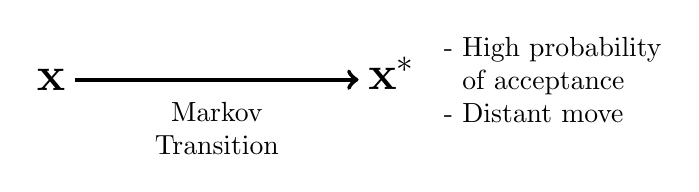
\begin{tikzpicture}[xscale=1.2, yscale=0.8]
		\draw [->, ultra thick]  (0,0) -- (3,0);
		\node[align=center, left] at (0,0) {\LARGE $\mathbf x$};
		\node[align=center, right] at (3,0.1) {\LARGE $\mathbf x^*$};
		\node[align=center, below] at (1.5,-.2) {Markov \\ Transition};
		\node[align=left, right] at (3.8,0)
		{
		- High probability \\ \hphantom{-} of acceptance \\
		- Distant move
		};
	\end{tikzpicture}
	\end{center}

\end{frame}

\begin{frame}{Hamiltonian dynamics}
	\begin{itemize}
		\item A reformulation of classical mechanics which describes motion through Hamilton's equations:
		\only<1-2>{
		\begin{align*}
			\begin{gathered}
				\frac{\text{d} \mathbf x}{\text{d} t} = \frac{\partial H}{\partial \mathbf p}
				\ \text{ and } \
				\frac{\text{d} \mathbf p}{\text{d} t} = -\frac{\partial H}{\partial \mathbf x},
			\end{gathered}
		\end{align*}
		where $H = H(\mathbf x, \mathbf p)$ is the Hamiltonian of the system (total energy), and $(\mathbf x, \mathbf p)$ are the position and momentum coordinates of the body in motion.
		}
		\only<3>{
		\begin{align*}
			\begin{gathered}
				\frac{\text{d} \mathbf x}{\text{d} t} = \frac{\partial H}{\partial \mathbf p} = \frac{\partial}{\partial \mathbf p} {\color{fu-red} K(\mathbf p)}
				\ \text{ and } \
				\frac{\text{d} \mathbf p}{\text{d} t} = -\frac{\partial H}{\partial \mathbf x} = -\frac{\partial}{\partial \mathbf x} {\color[HTML]{377EB8} U(\mathbf x)},
			\end{gathered}
		\end{align*}
		where $H = H(\mathbf x, \mathbf p)$ is the Hamiltonian of the system (total energy), and $(\mathbf x, \mathbf p)$ are the position and momentum coordinates of the body in motion.
		}

		\only<2>{
		\item In a closed system,
		\[
			H(\mathbf x, \mathbf p) =
			{\color{white}
			\underbrace{\color{black} K(\mathbf p)}_{\color{gray} \text{Kinetic energy}}
			{\color{black} +}
			\underbrace{\color{black} U(\mathbf x)}_{\color{gray} \text{Potential energy}}
			}
		\]
		}
		\only<3>{
		\item In a closed system,
		\[
			H(\mathbf x, \mathbf p) =
			{\color{white}
			\underbrace{\color{fu-red} K(\mathbf p)}_{\color{gray} \text{Kinetic energy}}
			{\color{black} +}
			\underbrace{\color[HTML]{377EB8} U(\mathbf x)}_{\color{gray} \text{Potential energy}}
			}
		\]
		}
	\end{itemize}
\end{frame}

\begin{frame}{Hamiltonian dynamics cont.}
	\vspace{-3mm}
	\begin{itemize}
		\item To describe the evolution of $\big(\mathbf x(t), \mathbf p(t)\big)$ from time $t$ to $t+T$, it is necessary to discretise time and split $T = L \cdot \epsilon$.

		\vspace{2mm}
		\begin{center}
		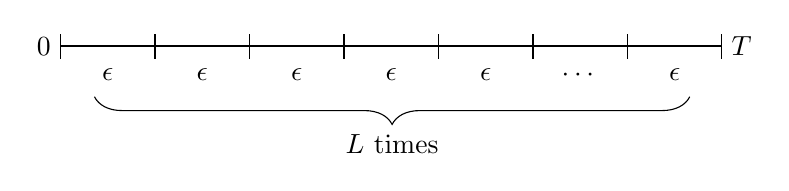
\begin{tikzpicture}[xscale=1.2, yscale=0.8]
			\draw [thick]  (0,0) -- (7,0);
			\foreach \x in  {0,1,2,3,4,5,6,7}
			\draw (\x,-.2) -- (\x, .2);
			\foreach \x in  {0.5,1.5,2.5,3.5,4.5}
			\node[align=center, below] at (\x,-.2) {$\epsilon$};
			\node[align=center, below] at (5.5,-.2) {$\cdots$};
			\node[align=center, below] at (6.5,-.2) {$\epsilon$};
			\node[align=center, left] at (0,0) {$0$};
			\node[align=center, right] at (7,0) {$T$};
			\draw[decorate, decoration={brace, mirror, amplitude=10pt}, xshift=-4pt, yshift=0pt]
			(0.5,-0.8) -- (6.8,-0.8) node [midway,below,yshift=-10pt] {$L$ times};
		\end{tikzpicture}
		\end{center}
		\vspace{-1.5mm}

		\pause
		\item Solve the system of differential equations using Euler's method, or the more commonly used leapfrog integration:
		\begin{align*}
			{\color{fu-red} \text{Step 1: }} &
			\mathbf p(t + \epsilon/2)
			= \mathbf p(t) - \frac{\epsilon}{2} \cdot \frac{\partial}{\partial \mathbf x} U \big( \mathbf x(t) \big)  \\
			{\color{fu-red} \text{Step 2: }} &
			\hphantom{/2} \mathbf x(t + \epsilon)
			=  \mathbf x(t) + \epsilon \cdot \frac{\partial}{\partial \mathbf p} K \big( \mathbf p(t + \epsilon / 2) \big)  \\
			{\color{fu-red} \text{Step 3: }} &
			 \hphantom{/2} \mathbf p(t + \epsilon)
			 = \mathbf p(t + \epsilon/2) - \frac{\epsilon}{2} \cdot \frac{\partial}{\partial \mathbf x} U \big( \mathbf x(t + \epsilon) \big)
		\end{align*}
		Steps 1-3 are repeated $L$ times.

	\end{itemize}
\end{frame}

\begin{frame}{Hamiltonian dynamics cont.}
	\begin{center}
	{\Huge Demo \\}
	\vspace{2em}
	\href{https://haziqjamil.shinyapps.io/hmc1/}{\texttt{https://haziqjamil.shinyapps.io/{\color{fu-red}hmc1}/}}	\end{center}
\end{frame}

\subsection{The HMC algorithm}

\begin{frame}{Probability and the Hamiltonian}
	\begin{itemize}
		\only<1-2>{
		\item Given some energy function $E(\boldsymbol\theta)$ over states $\boldsymbol\theta$, the \textit{canonical distribution} of the states $\boldsymbol\theta$ is given by the pdf
		\[
			f(\boldsymbol{\theta}) = \frac{1}{Z} \exp \left[ -\frac{E(\boldsymbol\theta)}{kT} \right].
		\]
		where $k$ is Boltzmann's constant, $T$ is the absolute temperature of the system, and $Z$ is a normalising constant.
		}
		\only<3-5>{
		\item {\color{gray!50} Given some energy function $E(\boldsymbol\theta)$ over states $\boldsymbol\theta$, the \textit{canonical distribution} of the states $\boldsymbol\theta$ is given by the pdf}
		\[
			f(\mathbf x, \mathbf p) = \frac{1}{Z} \exp \left[ -\frac{H(\mathbf x, \mathbf p)}{kT} \right].
		\]
		{\color{gray!50} where $k$ is Boltzmann's constant, $T$ is the absolute temperature of the system, and $Z$ is a normalising constant.}
		}

		\uncover<2->{
		\item The Hamiltonian $H(\mathbf x, \mathbf p) = K(\mathbf p) + U(\mathbf x)$ is one such energy function over states $(\mathbf x, \mathbf p)$.
		}

		\uncover<4->{
		\item Notice that the distribution for $\mathbf x$ and $\mathbf p$ are independent:
		\begin{align*}
			f(\mathbf x, \mathbf p) &\propto \exp \left[ -\frac{K(\mathbf p)}{kT} \right] \exp \left[ -\frac{U(\mathbf x)}{kT} \right] = f(\mathbf x) f(\mathbf p).
		\end{align*}
		}

		\uncover<5->{
		\item Typically, choose $T$ such that $kT = 1$.
		}
	\end{itemize}
\end{frame}

\begin{frame}{Choosing the energy functions}
	\begin{itemize}
		\item Using a \textit{quadratic kinetic energy function} $K(\mathbf p) = \mathbf p^\top \mathbf M^{-1} \mathbf p / 2$ yields a normal density function
		\begin{align*}
			f(\mathbf p) \propto \exp \left[ -\frac{1}{2} \mathbf p^\top \mathbf M^{-1} \mathbf p \right],
		\end{align*}
		implying $\mathbf p \sim \N_d(\mathbf 0, \mathbf M)$, where $\mathbf M = \text{diag}[m_1, \dots, m_d]$ is the mass matrix.

		\pause
		\item As for the potential energy, choose a function such that
		\[
			 U(\mathbf x) = -\log f(\mathbf x),
		\]
		since $f(\mathbf x) \propto \exp [ - U( \mathbf x)]$, where $f(\mathbf x)$ is the target density from which we wish to sample.

	\end{itemize}
\end{frame}

\begin{frame}{Hamiltonian Monte Carlo}
	\begin{itemize}
		\vspace{-3mm}
		\item To sample variables $\mathbf x$ , introduce momentum variables $\mathbf p$ and sample jointly from $f(\mathbf x, \mathbf p) = f(\mathbf x) f(\mathbf p)$.
		
		\pause
		\item The Hamiltonian Monte Carlo (HMC) algorithm

		\begin{adjustwidth}{0.6cm}{0.4cm}
		\begin{enumerate}[Step 1]
			\item \textit{Perturb momentum}. Draw $\mathbf p$ from $\N_d(\mathbf 0, \mathbf M)$.
			
			\pause
			\item \textit{Metropolis update}. Simulate Hamiltonian dynamics using $L$ leapfrogs of step-size $\epsilon$ and obtain a new state $(\mathbf x^*, \mathbf p^*)$. Accept the proposal state with probability $\min(1,A)$, where
			\begin{align*}
				A = \frac{f(\mathbf x^*, \mathbf p^*)}{f(\mathbf x, \mathbf p)}
				= \exp \left[ H(\mathbf x, \mathbf p) - H(\mathbf x^*, \mathbf p^*) \right].
			\end{align*}
		\end{enumerate}
		\end{adjustwidth}

	\end{itemize}

	\vspace{-10mm}
	
	\only<4>{
\begin{knitrout}\small
\definecolor{shadecolor}{rgb}{0.969, 0.969, 0.969}\color{fgcolor}

{\centering \includegraphics[width=\maxwidth]{figure/phaseportrait1-1} 

}



\end{knitrout}
	}
	
	\only<5>{
\begin{knitrout}\small
\definecolor{shadecolor}{rgb}{0.969, 0.969, 0.969}\color{fgcolor}

{\centering \includegraphics[width=\maxwidth]{figure/phaseportrait2-1} 

}



\end{knitrout}
	}
	
	\only<6>{
\begin{knitrout}\small
\definecolor{shadecolor}{rgb}{0.969, 0.969, 0.969}\color{fgcolor}

{\centering \includegraphics[width=\maxwidth]{figure/phaseportrait3-1} 

}



\end{knitrout}
	}

	\only<7>{
\begin{knitrout}\small
\definecolor{shadecolor}{rgb}{0.969, 0.969, 0.969}\color{fgcolor}

{\centering \includegraphics[width=\maxwidth]{figure/phaseportrait4-1} 

}



\end{knitrout}
	}
	
	\only<8>{
\begin{knitrout}\small
\definecolor{shadecolor}{rgb}{0.969, 0.969, 0.969}\color{fgcolor}

{\centering \includegraphics[width=\maxwidth]{figure/phaseportrait5-1} 

}



\end{knitrout}
	}

	\uncover<9>{
\begin{knitrout}\small
\definecolor{shadecolor}{rgb}{0.969, 0.969, 0.969}\color{fgcolor}

{\centering \includegraphics[width=\maxwidth]{figure/phaseportrait6-1} 

}



\end{knitrout}
	}
	
		
\end{frame}

\begin{frame}{Hamiltonian Monte Carlo cont.}
	\begin{center}
	{\Huge Demo \\}
	\vspace{2em}
	\href{https://haziqjamil.shinyapps.io/hmc2/}{\texttt{https://haziqjamil.shinyapps.io/{\color{fu-red}hmc2}/}}	\end{center}
\end{frame}

\subsection{HMC software}

\begin{frame}{Stan}
	\vspace{-5mm}
	\begin{figure}[hbt]
		\includegraphics[scale=0.25]{figure/mc-stan}
	\end{figure}
	\vspace{-5mm}

	\centering \url{http://mc-stan.org}
	\vspace{3mm}

	\begin{itemize}
%		\item Software for full Bayesian statistical inference with MCMC sampling using HMC.
		\item Stan interfaces: R, Python, shell, MATLAB, Julia, Stata, and Mathematica. Runs on Linux, Mac and Windows.
		\item R package \texttt{rstan} uses Stan modelling language. For expression-based Bayesian regression modelling, package \texttt{rstanarm} is available.
		\item Nice things about Stan
		\begin{itemize}
			\item Tuning is done automatically.
			\item Vast library of differentiable probability functions, or code your own.
			\item Conjugacy has no computational advantage.
			\item Optimising for efficiency possible, e.g. vectorisation.
		\end{itemize}
	\end{itemize}
\end{frame}

\newsavebox{\stana}
\begin{lrbox}{\stana}
\begin{knitrout}\footnotesize
\definecolor{shadecolor}{rgb}{0.969, 0.969, 0.969}\color{fgcolor}\begin{kframe}
\begin{alltt}
stan.iprior.mod <- "
  function \{
    ...
  \}
  data \{
    int n; // number of data
    int p; // number of parameters
    vector[n] Y; // responses
    matrix[n, p] X; // (centred) data
  \}
  transformed data \{
    matrix[p, p] XTX;
    XTX = X' * X;
  \}
  parameters \{
    real alpha;  // intercept
    real<lower=0> sigma;  // s.d. of errors
    vector[p] beta;  // regression coefficients
    vector<lower=0>[p] lambda;  // I-prior scale parameters
  \}
\end{alltt}
\end{kframe}
\end{knitrout}
\end{lrbox}

\newsavebox{\stanb}
\begin{lrbox}{\stanb}
\begin{knitrout}\footnotesize
\definecolor{shadecolor}{rgb}{0.969, 0.969, 0.969}\color{fgcolor}\begin{kframe}
\begin{alltt}
transformed parameters \{
  vector[p] lambdasq;
  cov_matrix[p] Sigma;
  vector[n] mu;
  lambdasq = lambda .* lambda;
  Sigma = \hlkwd{diag_matrix}(lambda) * XTX * \hlkwd{diag_matrix}(lambda) ./ (sigma ^ 2);
  mu = alpha + X * beta;
\}
model \{
  target += \hlkwd{inv_gamma_lpdf}(lambdasq | 0.0001, 0.0001);
  target += \hlkwd{multi_normal_lpdf}(beta | \hlkwd{rep_vector}(0, p), Sigma);
  target += \hlkwd{normal_lpdf}(Y | mu, sigma);
\}
generated quantities \{
  ...
\}
"
\end{alltt}
\end{kframe}
\end{knitrout}
\end{lrbox}



\newsavebox{\stancomp}
\begin{lrbox}{\stancomp}
\begin{knitrout}\small
\definecolor{shadecolor}{rgb}{0.969, 0.969, 0.969}\color{fgcolor}\begin{kframe}
\begin{alltt}
\hlstd{m} \hlkwb{<-} \hlkwd{stan_model}\hlstd{(}\hlkwc{model_code} \hlstd{= stan.mod)}
\hlstd{m}\hlopt{@}\hlkwc{model_name} \hlkwb{<-} \hlstr{"iprior"}
\end{alltt}
\end{kframe}
\end{knitrout}
\end{lrbox}

\newsavebox{\standata}
\begin{lrbox}{\standata}
\begin{knitrout}\small
\definecolor{shadecolor}{rgb}{0.969, 0.969, 0.969}\color{fgcolor}\begin{kframe}
\begin{alltt}
\hlstd{stan.dat} \hlkwb{<-} \hlkwd{list}\hlstd{(}\hlkwc{Y} \hlstd{=} \hlkwd{as.vector}\hlstd{(Y),} \hlkwc{X} \hlstd{= Xs,} \hlkwc{n} \hlstd{= n,} \hlkwc{p} \hlstd{= p)}
\end{alltt}
\end{kframe}
\end{knitrout}
\end{lrbox}

\newsavebox{\stansamp}
\begin{lrbox}{\stansamp}
\begin{knitrout}\small
\definecolor{shadecolor}{rgb}{0.969, 0.969, 0.969}\color{fgcolor}\begin{kframe}
\begin{alltt}
\hlstd{fit.stan} \hlkwb{<-} \hlkwd{stan}\hlstd{(}\hlkwc{model_code} \hlstd{= stan.mod,} \hlkwc{data} \hlstd{= stan.dat,}
                 \hlkwc{pars} \hlstd{=} \hlkwd{c}\hlstd{(}\hlstr{"alpha"}\hlstd{,} \hlstr{"beta"}\hlstd{,} \hlstr{"lambda"}\hlstd{,} \hlstr{"sigma"}\hlstd{),}
                 \hlkwc{iter} \hlstd{=} \hlnum{50000}\hlstd{,} \hlkwc{chains} \hlstd{=} \hlnum{4}\hlstd{,} \hlkwc{thin} \hlstd{=} \hlnum{10}\hlstd{)}
\end{alltt}
\end{kframe}
\end{knitrout}
\end{lrbox}

\newsavebox{\stanres}
\begin{lrbox}{\stanres}
\begin{knitrout}\footnotesize
\definecolor{shadecolor}{rgb}{0.969, 0.969, 0.969}\color{fgcolor}\begin{kframe}
\begin{alltt}
\hlkwd{print}\hlstd{(fit.stan)}
\end{alltt}
\begin{verbatim}
## Inference for Stan model: iprior.
## 4 chains, each with iter=50000; warmup=25000; thin=10; 
## post-warmup draws per chain=2500, total post-warmup draws=10000.
## 
##              mean se_mean   sd    2.5%     25%     50%     75%   97.5%
## alpha       -1.04    0.00 0.19   -1.40   -1.16   -1.04   -0.92   -0.68
## beta[1]      9.71    0.00 0.20    9.32    9.58    9.71    9.84   10.10
## beta[2]      0.07    0.00 0.10   -0.10    0.01    0.06    0.12    0.31
## lambda[1]    2.26    0.03 2.55    0.70    1.14    1.61    2.47    7.78
## lambda[2]    0.03    0.00 0.06    0.01    0.01    0.02    0.03    0.09
## sigma        1.91    0.00 0.13    1.68    1.82    1.91    2.00    2.20
## lp__      -224.20    0.02 1.85 -228.60 -225.24 -223.88 -222.82 -221.62
##           n_eff Rhat
## alpha     10000    1
## beta[1]   10000    1
## beta[2]    9410    1
## lambda[1] 10000    1
## lambda[2]  9972    1
## sigma     10000    1
## lp__      10000    1
## 
## Samples were drawn using NUTS(diag_e) at Sat Oct 29 01:19:21 2016.
## For each parameter, n_eff is a crude measure of effective sample size,
## and Rhat is the potential scale reduction factor on split chains (at 
## convergence, Rhat=1).
\end{verbatim}
\end{kframe}
\end{knitrout}
\end{lrbox}


\begin{frame}[fragile]{Stan example}
	\only<1>{\vspace{-2mm} \usebox{\stana}}
	\only<2>{\vspace{-2mm} \usebox{\stanb}}
	
	\only<3-5>{
		\begin{itemize}
			\item Compile the Stan model.
		\end{itemize}
		\usebox{\stancomp}
	}
	
	\only<4-5>{
		\begin{itemize}
			\item Set the data for Stan to use.
		\end{itemize}
		\usebox{\standata}
	}
	
	\only<5-5>{
		\begin{itemize}
			\item Begin sampling
		\end{itemize}
		\usebox{\stansamp}
	}
	
	\only<6>{\vspace{-1mm} \usebox{\stanres}}
	
	\only<7>{
\begin{knitrout}\small
\definecolor{shadecolor}{rgb}{0.969, 0.969, 0.969}\color{fgcolor}

{\centering \includegraphics[width=1.05\linewidth]{figure/stanplot-1} 

}



\end{knitrout}
	}
	
	\only<8>{
\begin{knitrout}\small
\definecolor{shadecolor}{rgb}{0.969, 0.969, 0.969}\color{fgcolor}

{\centering \includegraphics[width=1.05\linewidth]{figure/lambdastan-1} 

}



\end{knitrout}
	}
		
\end{frame}

\begin{frame}{HMC unable to sample from discrete distributions}
	\begin{itemize}
		\item HMC requires that the domain of $f(\mathbf x)$ is continuous and $\partial \log f(\mathbf x) / \partial \mathbf x$ is inexpensive to compute.

		\item This is a problem for our Bayesian Variable Selection model because we need posterior samples of $\boldsymbol{\gamma} \in \{0,1\}^p$.

		\item Three ideas:
		\begin{itemize}
			\item Marginalise the discrete variables.
			\item Use an underlying latent continuous variable.
			\item Augment with Gibbs sampling.
		\end{itemize}

	\end{itemize}

\end{frame}

\begin{frame}{Approach 1: Marginalise}
	\vspace{-2mm}
	\begin{itemize}
		\item Let $\boldsymbol{\theta}$ be some continuous parameters and $\boldsymbol{\gamma}$ be some discrete parameters in the model with data $\mathbf y$.
		\item Since unable to sample from $f(\boldsymbol{\gamma} | \mathbf y)$, integrate out $\boldsymbol{\gamma}$ from the model, and just sample from the posterior of $\boldsymbol{\theta}$
		\[
			f(\boldsymbol{\theta} | \mathbf y) = \sum_{\boldsymbol\gamma} f(\boldsymbol{\theta}, \boldsymbol\gamma | \mathbf y)
			= f(\boldsymbol\theta) \sum_{\boldsymbol\gamma}  f(\mathbf y | \boldsymbol{\theta}, \boldsymbol\gamma)f(\boldsymbol\gamma)
		\]
		\item The unnormalised posterior probability mass function for $\boldsymbol\gamma$ is
		\[
			q(\boldsymbol{\gamma}) = \frac{1}{M} \sum_{m=1}^M f(\boldsymbol{\theta}^{(m)}, \boldsymbol\gamma | \mathbf y)
		\]
		where $m = 1, \dots, M$ is the index for the posterior draws.

		\item Problem: For Bayesian Variable Selection models, this is intractable because need to sum over all $2^p$ models.
	\end{itemize}
\end{frame}

\begin{frame}{Approach 2: Latent continuous variables}
	\begin{itemize}
		\item For the Bayesian Variable Selection model, assume there is underlying standard normal random variable $Z_j$ for each $j = 1,\dots,p$ such that
		\begin{align*}
			\gamma_j =
			\begin{cases}
				1	&Z_j \geq 0\\
				0	&Z_j < 0\\
			\end{cases}
		\end{align*}
		\item Probabilities are preserved: $\P[\gamma_j = 1] = \P[Z_j \geq 0] = 0.5$.
		\item Problems:
		\begin{itemize}
			\item Does this make sense?
			\item The discrete variables still ``exist'', so possibly derivatives will break.
		\end{itemize}
	\end{itemize}
\end{frame}

\begin{frame}{Approach 3: Use Gibbs sampler}
	\begin{itemize}
		\item Sample the continuous parameters $\boldsymbol\theta$ using HMC.
		\item At each iteration $m$, use $\boldsymbol\theta^{(m)}$ in the Gibbs conditional densities to sample $\boldsymbol{\gamma}$.
		\item Problem: Have to write code for the HMC sampler, which won't include all the automatic tuning that Stan has.
	\end{itemize}
\end{frame}

%%%%%%%%%%%%%%%%%%%%%%%%%%%%%%%%%%%%%%%%%%%%%%%%%%%%%%%%%%%%%%%%%%%%%%%%%%%%%%%%
\section{Summary} %%%%%%%%%%%%%%%%%%%%%%%%%%%%%%%%%%%%%%%%%%%%%%%%%%%%%%%%%%%%%%
%%%%%%%%%%%%%%%%%%%%%%%%%%%%%%%%%%%%%%%%%%%%%%%%%%%%%%%%%%%%%%%%%%%%%%%%%%%%%%%%

{
\framenonumber
\begin{frame}[noframenumbering]
	\tableofcontents[currentsection, sections=1-5, hideallsubsections]
\end{frame}
}

\begin{frame}{Summary}
	\begin{itemize}
		\item For our I-prior Bayesian Variable Selection model
		\begin{itemize}
			\item Promising results in both simulated and real-world data.
			\item The individual scale parameters $\lambda_1,\dots,\lambda_p$ are important.
			\item We have used ML estimate for $\boldsymbol{\lambda}$ in our Bayesian model.
		\end{itemize}
		\item Things I want to do
		\begin{itemize}
			\item Any model consistency results for Bayesian variable selection models?
			\item Any mathematical justification as to why we should use individual scale parameters?
			\item How does the off-diagonal elements in the I-prior covariance matrix help things?
		\end{itemize}
		\item Wishlist: Make HMC work for Bayesian variable selection models.
	\end{itemize}
\end{frame}

\begin{frame}{What we've seen today}
	\begin{enumerate}[1]
		\item I-prior models estimated using ML methods (EM algorithm) and use of the \texttt{iprior} package in R.
%		\item \texttt{lme4} style of estimating mixed-effects models using sparse Cholesky decomposition.
		\item Shrinkage properties of I-priors for use in Bayesian variable selection.
		\item Bayesian estimation in JAGS.
		\item Shiny apps for reactive programming.
		\item Hamiltonian dynamics and Hamiltonian Monte Carlo.
		\item Bayesian inference using HMC via Stan.
		\item \texttt{knitr} for combining (evaluated) R code and plots into documents.
		\item Git and GitHub for version control.
	\end{enumerate}
\end{frame}

\begin{frame}[fragile, label=c]
\frametitle[knitr example]{\texttt{knitr} example}

	\begin{itemize}
		\item You type:
	\end{itemize}
\texttt{<<chunk.name, echo = TRUE>>=} \\
\texttt{x <- rnorm(100)} \\
\texttt{max(x)} \\
\texttt{hist(x)} \\
\texttt{@}

	\begin{itemize}
		\item The output:
	\end{itemize}
	
	\vspace{-5mm}
	\begin{columns}
		\begin{column}{0.5\textwidth}
\begin{knitrout}\small
\definecolor{shadecolor}{rgb}{0.969, 0.969, 0.969}\color{fgcolor}\begin{kframe}
\begin{alltt}
\hlstd{x} \hlkwb{<-} \hlkwd{rnorm}\hlstd{(}\hlnum{100}\hlstd{)}
\hlkwd{max}\hlstd{(x)}
\end{alltt}
\begin{verbatim}
## [1] 2.375356
\end{verbatim}
\end{kframe}
\end{knitrout}
		\vspace{18mm}
		\end{column}
		\begin{column}{0.5\textwidth}
\begin{knitrout}\small
\definecolor{shadecolor}{rgb}{0.969, 0.969, 0.969}\color{fgcolor}\begin{kframe}
\begin{alltt}
\hlkwd{hist}\hlstd{(x)}
\end{alltt}
\end{kframe}

{\centering \includegraphics[width=1\linewidth]{figure/chunk_name2-1} 

}



\end{knitrout}
		\end{column}
	\end{columns}

\end{frame}

%%%%%%%%%%%%%%%%%%%%%%%%%%%%%%%%%%%%%%%%%%%%%%%%%%%%%%%%%%%%%%%%%%%%%%%%%%%%%%%%
%%% BIBLIOGRAPHY %%%%%%%%%%%%%%%%%%%%%%%%%%%%%%%%%%%%%%%%%%%%%%%%%%%%%%%%%%%%%%%
%%%%%%%%%%%%%%%%%%%%%%%%%%%%%%%%%%%%%%%%%%%%%%%%%%%%%%%%%%%%%%%%%%%%%%%%%%%%%%%%

{\framenonumber
\begin{frame}[t,allowframebreaks,noframenumbering]{References}	
	\bibliographystyle{apalike}
	\nocite{*}
	\bibliography{soc-stat-meet}
\end{frame}
}

{\framenonumber
\begin{frame}[t,allowframebreaks,noframenumbering]{HMC References}	
	\bibliographystyleHMC{apalike}
	\nociteHMC{*}
	\bibliographyHMC{soc-stat-hmc}	
\end{frame}
}

{\framenonumber
\begin{frame}[t,allowframebreaks,noframenumbering]{Stuff}	
	\bibliographystyleTools{apalike}
	\nociteTools{*}
	\bibliographyTools{soc-stat-tools}	
\end{frame}
}

%%%%%%%%%%%%%%%%%%%%%%%%%%%%%%%%%%%%%%%%%%%%%%%%%%%%%%%%%%%%%%%%%%%%%%%%%%%%%%%%
\section{End} %%%%%%%%%%%%%%%%%%%%%%%%%%%%%%%%%%%%%%%%%%%%%%%%%%%%%%%%%%%%%%%%%%
%%%%%%%%%%%%%%%%%%%%%%%%%%%%%%%%%%%%%%%%%%%%%%%%%%%%%%%%%%%%%%%%%%%%%%%%%%%%%%%%

{
\framenonumber
\begin{frame}[noframenumbering]{End}
\begin{center}
\Huge Thank you!
\end{center}
\end{frame}
}

%%%%%%%%%%%%%%%%%%%%%%%%%%%%%%%%%%%%%%%%%%%%%%%%%%%%%%%%%%%%%%%%%%%%%%%%%%%%%%%%
\appendix %%%%%%%%%%%%%%%%%%%%%%%%%%%%%%%%%%%%%%%%%%%%%%%%%%%%%%%%%%%%%%%%%%%%%%
\beginbackup %%%%%%%%%%%%%%%%%%%%%%%%%%%%%%%%%%%%%%%%%%%%%%%%%%%%%%%%%%%%%%%%%%%
%%%%%%%%%%%%%%%%%%%%%%%%%%%%%%%%%%%%%%%%%%%%%%%%%%%%%%%%%%%%%%%%%%%%%%%%%%%%%%%%

{
\framenonumber
\begin{frame}[noframenumbering]
	\tableofcontents[sections=6]
\end{frame}
}

%%%%%%%%%%%%%%%%%%%%%%%%%%%%%%%%%%%%%%%%%%%%%%%%%%%%%%%%%%%%%%%%

\section{Additional material}

\subsection[lme4 methods]{\texttt{lme4} methods}

\begin{frame}{Minimising profiled deviance (à la \texttt{lme4})}
	\begin{itemize}
		\item Very fast algorithm to obtain MLEs of mixed-effects models by using sparse Cholesky decomposition.
		\item Consider the mixed-effects model
		\begin{align*}
			\begin{gathered}
				\mathbf y = \mathbf X\boldsymbol{\beta} + \mathbf Z\mathbf b + \boldsymbol{\epsilon} \\
				\boldsymbol{\epsilon} \sim \N (\mathbf 0, \sigma^2 \mathbf I_n) \\
				\mathbf b \sim \N (\mathbf 0, \boldsymbol{\Sigma})
			\end{gathered}
		\end{align*}
		\item Suppose that $\boldsymbol{\Sigma} = \sigma^2\boldsymbol{\Lambda}_{\boldsymbol{\theta}}\boldsymbol{\Lambda}_{\boldsymbol{\theta}}^\top$. Then the following model is equivalent, where we have used the subsitution $\mathbf b = \boldsymbol{\Lambda}_{\boldsymbol{\theta}}\mathbf u$:
		\begin{align*}
			\begin{gathered}
				\mathbf y = \mathbf X\boldsymbol{\beta} + \mathbf Z\boldsymbol{\Lambda}_{\boldsymbol{\theta}}\mathbf u + \boldsymbol{\epsilon} \\
				\boldsymbol{\epsilon} \sim \N (\mathbf 0, \sigma^2 \mathbf I_n) \\
				\mathbf u \sim \N (\mathbf 0, \sigma^2 \mathbf I_n)
			\end{gathered}
		\end{align*}
	\end{itemize}
\end{frame}

\begin{frame}{Minimising profiled deviance (à la \texttt{lme4}) cont.}
	\begin{itemize}
		\only<1>{
		\item The density of interest is $f(\mathbf y) = \int h(\mathbf u) \,\text{d}\mathbf u$, where
		\begin{align*}
			h(\mathbf u) &= f(\mathbf y | \mathbf u) f(\mathbf u) \\
			&= (2\pi\sigma^2)^{-(n+q)/2} \exp \left[- \frac{\Vert \mathbf y - \mathbf X\boldsymbol\beta - \mathbf Z\boldsymbol{\Lambda}_{\boldsymbol{\theta}}\mathbf u \Vert^2 + \Vert \mathbf u \Vert^2}{2\sigma^2} \right]
		\end{align*}
		}

		\only<2>{
		\item The density of interest is $f(\mathbf y) = \int h(\mathbf u) \,\text{d}\mathbf u$, where
		\begin{align*}
			h(\mathbf u) &= f(\mathbf y | \mathbf u) f(\mathbf u) \\
			&= (2\pi\sigma^2)^{-(n+q)/2} \exp \left[- \frac{{\color{fu-red} \Vert \mathbf y - \mathbf X\boldsymbol\beta - \mathbf Z\boldsymbol{\Lambda}_{\boldsymbol{\theta}}\mathbf u \Vert^2 + \Vert \mathbf u \Vert^2}}{2\sigma^2} \right]
		\end{align*}
		}

		\uncover<2->{
		\item Each calculation of $f(\mathbf y)$ involves obtaining the conditional modes
			\[
				\tilde{\mathbf u}(\boldsymbol\theta, \boldsymbol\beta) = \mathop{\arg\min}_{\mathbf u} {\color{fu-red} d(\mathbf u, \boldsymbol\theta, \boldsymbol\beta)}
			\]
			by computing the sparse Cholesky factorisation
			\[
				\mathbf L_{\boldsymbol{\theta}} \mathbf L_{\boldsymbol{\theta}}^\top = \boldsymbol{\Lambda}_{\boldsymbol{\theta}}^\top \mathbf Z ^\top \mathbf Z \boldsymbol{\Lambda}_{\boldsymbol{\theta}} + \mathbf I_q,
			\]
			and solving $\mathbf L_{\boldsymbol{\theta}}^\top \tilde{\mathbf u} = c(\boldsymbol\theta, \boldsymbol\beta)$ by back substitution.
		}
	\end{itemize}
\end{frame}

\begin{frame}{Minimising profiled deviance (à la \texttt{lme4}) cont.}
	\begin{itemize}
		\item For linear mixed models, $f(\mathbf y) = \int h(\mathbf u) \,\text{d}\mathbf u$ has a closed-form expression in terms of $\mathbf L_{\boldsymbol{\theta}}$ and $\tilde{\mathbf u}(\boldsymbol\theta, \boldsymbol\beta)$:
			\begin{align}\label{eq:lme4dev}
				f(\mathbf y) = (2\pi\sigma^2)^{-n/2} \vert \mathbf L_{\boldsymbol{\theta}} \vert^{-1} \exp \left[- \frac{d ( \tilde{\mathbf u}, \boldsymbol\theta, \boldsymbol\beta)}{2\sigma^2} \right].
			\end{align}
		\item On the deviance scale, we have $D(\boldsymbol\theta, \boldsymbol\beta, \sigma) = -2 \log f(\mathbf y)$. The value of $\sigma$ which minimises the deviance is
			\[
				\sigma^2(\boldsymbol\theta, \boldsymbol\beta) = \frac{d ( \tilde{\mathbf u}, \boldsymbol\theta, \boldsymbol\beta)}{n}.
			\]
		\item Plugging this back into \eqref{eq:lme4dev}, we obtain the profiled deviance
			\[
				D(\boldsymbol\theta, \boldsymbol\beta) = 2 \log \vert \mathbf L_{\boldsymbol{\theta}} \vert + n \left( 1 + \log \left(2\pi \frac{d ( \tilde{\mathbf u}, \boldsymbol\theta, \boldsymbol\beta)}{n} \right)\right)
			\]
			which is then minimised to obtain MLEs $\hat{\boldsymbol\theta}$, $\hat{\boldsymbol\beta}$ and $\sigma^2(\hat{\boldsymbol\theta}, \hat{\boldsymbol\beta})$.
	\end{itemize}
\end{frame}

\begin{frame}{Minimising profiled deviance (à la \texttt{lme4}) cont.}
	\vspace{-1mm}
	\begin{itemize}
		\item ``Eliminate'' fixed effects $\boldsymbol{\beta}$.
		\begin{itemize}
			\item Find conditional modes $\tilde{\boldsymbol{\beta}}(\boldsymbol\theta)$
			\begin{align*}
				\begin{pmatrix}
					\tilde{\mathbf u}(\boldsymbol\theta) \\
					\tilde{\boldsymbol{\beta}}(\boldsymbol\theta)
				\end{pmatrix}
				=
				\mathop{\arg\min}_{(\mathbf u, \boldsymbol{\beta})} d(\mathbf u, \boldsymbol\beta, \boldsymbol\theta)
			\end{align*}
			via a sparse Cholesky decomposition. Following a similar method as before, obtain a profiled deviance which depends only on $\boldsymbol{\theta}$
			\[
				D(\boldsymbol\theta) = 2 \log \vert \mathbf L_{\boldsymbol{\theta}} \vert + n \left( 1 + \log \left(2\pi \frac{d ( \tilde{\mathbf u}, \boldsymbol\theta, \tilde{\boldsymbol\beta})}{n} \right)\right).
			\]

			\pause
			\item In addition, use the restricted maximum likelihood (REML) criterion
			\[
				D_R(\boldsymbol\theta, \sigma) = -2 \log \int f(\mathbf y) \,\text{d} \boldsymbol\beta.
			\]
			Again, follow similar steps to obtain the profiled REML criterion
			\[
				D_R(\boldsymbol\theta) = 2 \log (\vert \mathbf L_{\boldsymbol{\theta}} \vert \mathbf L_{\mathbf X} \vert ) + (n - p) \left( 1 + \log \left(2\pi \frac{d ( \tilde{\mathbf u}, \boldsymbol\theta, \tilde{\boldsymbol\beta})}{n-p} \right)\right).
			\]
		\end{itemize}
	\end{itemize}
\end{frame}

\begin{frame}{Coerce the $w$ I-prior model into a mixed-model}
	\vspace{-5mm}
	\begin{align*}
	\mathbf y &= \boldsymbol{\alpha} + (\lambda_1\mathbf H_1 + \dots + \lambda_p\mathbf H_p) \mathbf w + \boldsymbol{\epsilon} \\
	&=
	{\color{gray}
	\underbrace{ \color{black}
	\begin{bmatrix}
		1 \\
		\vdots \\
		1
	\end{bmatrix}
	}_{\mathbf X}
	\underbrace{\color{black} \vphantom{\begin{bmatrix} 1 \\ \vdots \\ 1 \end{bmatrix}}
	\begin{bmatrix}
		\alpha
	\end{bmatrix}
	}_{\boldsymbol{\beta}}
	+
	\underbrace{\color{black} \vphantom{\begin{bmatrix} 1 \\ \vdots \\ 1 \end{bmatrix}}
	\begin{bmatrix}
		\mathbf H_1	&\cdots	&\mathbf H_p
	\end{bmatrix}
	}_{\mathbf Z}
	\underbrace{\color{black}
	\begin{bmatrix}
		\lambda_1\mathbf I_n \\
		\vdots \\
		\lambda_p\mathbf I_n
	\end{bmatrix}
	}_{\boldsymbol{\Lambda}_{\boldsymbol{\lambda}}}
	}
	\mathbf w + \boldsymbol{\epsilon} \\
	&= \mathbf X \boldsymbol{\beta} + \mathbf Z \boldsymbol{\Lambda}_{\boldsymbol{\lambda}} \mathbf w + \boldsymbol{\epsilon} \\
	&= \mathbf X \boldsymbol{\beta} + \mathbf Z
		{\color{gray}
		\underbrace{\color{black} \left(\frac{1}{\sigma^2}\boldsymbol{\Lambda}_{\boldsymbol{\lambda}}\right)}_{\boldsymbol{\Lambda}_{\boldsymbol{\theta}}}
		\underbrace{\color{black} \vphantom{\left(\frac{1}{\sigma^2}\boldsymbol{\Lambda}_{\boldsymbol{\lambda}}\right)}
		(\sigma^2 \mathbf w)}_{\mathbf u}
		} + \boldsymbol{\epsilon} \\
	&=  \mathbf X \boldsymbol{\beta} + \mathbf Z \boldsymbol{\Lambda}_{\boldsymbol{\theta}} \mathbf u + \boldsymbol{\epsilon}
	\end{align*}

	\begin{itemize}
		\item Our scale parameters are contained in $\boldsymbol{\theta}=(\lambda_1/\sigma^2, \dots, \lambda_p/\sigma^2)$.
		\item Problem: Our $\mathbf Z$ matrix is dense, so not able to use sparse Cholesky methods.
	\end{itemize}
\end{frame}

\subsection{MLE vs Bayes for scale parameters}

\begin{frame}{MLE vs Bayes for scale parameters}
	\begin{itemize}
		\item For each $k = 1,\dots,p$, the maximum a posteriori (MAP) estimate is
		\begin{align*}
			\hat\lambda_k^{MAP} &= \mathop{\arg\max}_{\lambda_k} f(\alpha, \boldsymbol{\beta}, \psi, \boldsymbol{\lambda} | \mathbf y)
 \\
			&= \mathop{\arg\max}_{\lambda_k} f(\mathbf y , \boldsymbol{\beta} | \alpha, \psi, \boldsymbol{\lambda}) f(\psi) f(\lambda_1)\cdots f(\lambda_p) \\
			&= \mathop{\arg\max}_{\lambda_k} f(\mathbf y , \boldsymbol{\beta} | \alpha, \psi, \boldsymbol{\lambda}) f(\lambda_k)
		\end{align*}
		whereas the ML estimate is
		\begin{align*}
			\hat\lambda_k^{ML} &= \mathop{\arg\max}_{\lambda_k} f(\mathbf y; \boldsymbol\lambda, \psi) \\
			&= \mathop{\arg\max}_{\lambda_k} \int f(\mathbf y, \boldsymbol\beta ; \boldsymbol\lambda, \psi) \, \text{d}\boldsymbol\beta
		\end{align*}

		\item $\hat\lambda_k^{MAP} = \hat\lambda_k^{ML}$ if the beta I-prior model is marginalised over $\boldsymbol{\beta}$, and a uniform prior is used for each $\lambda_k$.
	\end{itemize}
\end{frame}

\backupend

\end{document}
